% ---------------------------------------------------------------------------
% IT5006 Fundamentals of Data Analytics
% Group Project Milestone 1: Literature Review and Exploratory Data Analysis
%
% Compiles with pdfLaTeX on Overleaf. Build order: pdflatex -> bibtex -> pdflatex x2
% ---------------------------------------------------------------------------
\documentclass[11pt,a4paper]{article}

\usepackage{lmodern}      % scalable Type 1 font; required for microtype expansion
\usepackage[T1]{fontenc}
\usepackage[utf8]{inputenc}
\usepackage[margin=1in]{geometry}
\usepackage{graphicx}
\usepackage{booktabs}
\usepackage{caption}
\usepackage{subcaption}
\usepackage{amsmath}
\usepackage{tikz}
\usetikzlibrary{arrows.meta}
\usepackage{microtype}
\usepackage{xcolor}
\usepackage[numbers,sort&compress]{natbib}
\usepackage[hidelinks]{hyperref}

\graphicspath{{figures/}}
% --- Citation marks -------------------------------------------------------
% Render the bracketed reference number one step smaller than the body text so
% it reads as a reference mark rather than competing with the prose.
\makeatletter
\renewcommand\NAT@open{\bgroup\footnotesize[}
\renewcommand\NAT@close{]\egroup}
\makeatother

% --- Footnotes ------------------------------------------------------------
% Lettered markers keep explanatory notes visually distinct from the numeric
% citation marks, and a full-width rule separates them from the body.
\renewcommand{\thefootnote}{\alph{footnote}}
\renewcommand{\footnoterule}{%
  \kern-3pt\hrule width \textwidth height 0.4pt\kern 4pt}
\setlength{\footnotesep}{0.62em}
\setlength{\skip\footins}{12pt plus 3pt minus 2pt}
% Note text sits a step below the citation marks, so the two never compete.
\makeatletter
\long\def\@makefntext#1{%
  \parindent 1em\noindent\hb@xt@1.6em{\hss\@makefnmark}\scriptsize #1}
\makeatother

% Tighter heading spacing: the default skips waste roughly a page across a
% document with this many subsections.
\usepackage{titlesec}
\titlespacing*{\section}{0pt}{1.5ex plus .3ex minus .2ex}{0.9ex}
\titlespacing*{\subsection}{0pt}{1.2ex plus .2ex minus .2ex}{0.5ex}
\titlespacing*{\paragraph}{0pt}{1.0ex plus .2ex}{1em}
\titleformat{\section}{\normalfont\large\bfseries}{\thesection}{0.7em}{}
\titleformat{\subsection}{\normalfont\normalsize\bfseries}{\thesubsection}{0.6em}{}

\usepackage[inline]{enumitem}
\setlist[enumerate]{topsep=3pt, itemsep=1.5pt, parsep=0pt, partopsep=0pt, leftmargin=1.5em}
\setlist[itemize]{topsep=3pt, itemsep=1.5pt, parsep=0pt, partopsep=0pt, leftmargin=1.4em}

\captionsetup{font=small,labelfont=bf,skip=5pt}
\setlength{\parskip}{0.10em}
% Tighten float separation so the body respects the 4-5 page limit.
\setlength{\textfloatsep}{10pt plus 2pt minus 2pt}
\setlength{\intextsep}{10pt plus 2pt minus 2pt}
\bibliographystyle{plainnat}

% Compact table column for the audit tables
\newcommand{\code}[1]{\texttt{\small #1}}

% ---------------------------------------------------------------------------
\begin{document}

% ============================== COVER PAGE =================================
\begin{titlepage}
\centering
\vspace*{3.5cm}

{\Large\bfseries Group Project Milestone 1:\par}
\vspace{0.6em}
{\Large\bfseries Literature Review and Exploratory Data Analysis\par}

\vspace{1.2cm}
{\large Forecasting Weekly Demand for Broadway Productions\par}
\vspace{0.4em}
{\normalsize A transactional analytics study of 26 years of box-office data\par}

\vspace{3.5cm}

% ---------------------------------------------------------------------------
% TODO before submission: replace with the real team roster.
% ---------------------------------------------------------------------------
{\normalsize
\begin{tabular}{ll}
Group & \textit{Group \_\_} \\[2pt]
Member 1 & \textit{Name (Student ID)} \\
Member 2 & \textit{Name (Student ID)} \\
Member 3 & \textit{Name (Student ID)} \\
Member 4 & \textit{Name (Student ID)} \\
Member 5 & \textit{Name (Student ID)} \\
\end{tabular}\par}

\vfill

{\large National University of Singapore\par}
\vspace{0.4em}
{\large IT5006 Fundamentals of Data Analytics\par}
\vspace{0.4em}
{\large AY2026/2027 Semester 1\par}

\vspace{1.2cm}
\end{titlepage}

% ============================== BODY =======================================
\section{Literature Review}

\subsection{Scope and domain framing}

This project analyses \emph{Broadway weekly grosses}: 29{,}167 weekly
box-office records covering 820 shows across 56 Manhattan theatres between
August 1990 and August 2016 \citep{corgis2016broadway}.\footnote{%
\textbf{Note on the data source.} The brief's Dataset section is written around
the Olist e-commerce tables, but the file distributed via Canvas is
\code{broadway\_clean.csv}. We follow its instruction to ``use this exact copy
rather than downloading it yourself from Kaggle or elsewhere'', which exists so
results stay comparable across teams. \emph{No external data was obtained}: the
Canvas file is the only source, and every target and feature here is derivable
from it alone.}
The project brief is written around e-commerce analytics, and the dataset
assigned to this group sits in an adjacent domain: live entertainment. We treat the brief's requirements as
domain-general, because the analytical structure is the same in both settings.
Both produce a stream of transactional records at a fixed reporting grain; both
raise questions of demand forecasting, revenue management and product-lifecycle
risk; and both are exposed to the same two methodological hazards the brief
emphasises, namely target leakage from post-outcome columns and misleading
accuracy on imbalanced targets. Where the brief gives an e-commerce example we
state the Broadway equivalent explicitly. The brief's warning about
\code{customer\_id} versus \code{customer\_unique\_id}, for instance, maps onto
the distinction between a weekly row and a \emph{production}: a long-running
show contributes hundreds of rows, so the grouping unit for any split must be
the production, not the row.

\subsection{Demand and success factors for cultural products}

The economics of Broadway has an established quantitative literature, and it is
unusually relevant here because it studies the same institution that generated
our data. \citet{reddy1998broadway} model show success as a function of critical
reviews, previews, advertising, ticket prices, show type and the timing of the
opening, and find that newspaper critics exert a large and asymmetric influence.
\citet{simonoff2003broadway} reframe success as \emph{longevity} and fit Cox
proportional-hazards models \citep{cox1972regression} to show survival, finding
that show type, revival status and first-week attendance are predictive, while a
Tony nomination matters far less than a Tony win. \citet{simonoff2016survival}
extend this with a three-way comparison of logistic regression, proportional
hazards and censored linear regression on the same underlying question,
confirming persistent positive effects of attendance and awards and showing that
musicals outlast comparable non-musicals.

Two lessons carry into our scoping. First, the strongest predictors in this
literature --- reviews, awards, advertising, casting --- are \emph{not present}
in our dataset, which holds only weekly box-office aggregates; any performance
ceiling we report must be read against that limitation. Second, survival framing
with explicit censoring is the established treatment for run length, rather than
naive regression on observed duration. The wider literature agrees:
\citet{sharda2006boxoffice} treat motion-picture box office as classification
over discretised revenue bands rather than point regression, because the
conditional distribution is wide and heavy-tailed, making a band prediction both
more attainable and more actionable.

\subsection{Modelling approaches for tabular panel data}

For tabular data of this size the practical model space is well characterised.
Regularised linear and logistic models remain the natural baseline: cheap,
interpretable, and revealing of distribution shift. Tree ensembles are the usual
step up --- \citet{breiman2001rf} bag decorrelated trees to cut variance, while
gradient boosting \citep{friedman2001gbm} and its scalable implementations
\citep{chen2016xgboost} fit residuals stagewise with shrinkage and explicit
complexity penalties. \citet{grinsztajn2022tabular} benchmark both families
against modern deep architectures across 45 datasets and find tree-based methods
still state-of-the-art at our scale, attributing the gap to inductive biases
better matched to irregular tabular targets. We therefore plan a deliberately
small model budget --- linear/logistic baselines, a regularised variant, one
tree ensemble --- reused across both framings, following the brief's guidance to
justify complexity with evidence rather than enumerate algorithms.

\subsection{Feature engineering for transactional panel data}

Panel data of this shape rewards a standard vocabulary: lagged target values,
rolling means and dispersions, trend differences, and calendar encodings
\citep{hyndman2021fpp}. Two refinements matter here. High-cardinality
categoricals such as our 56 theatres are poorly served by one-hot encoding;
target encoding \citep{miccibarreca2001target} compresses them while retaining
signal, provided it is fitted inside the cross-validation loop. And the lag
window must be tied to the decision it supports: a feature from week $t-1$ is
unavailable to a planner committing spend four weeks out, so the admissible lag
block is a function of the forecast horizon, not a free hyperparameter.

Leakage is the dominant risk. \citet{kaufman2012leakage} formalise it as the
introduction of information about the target that would not legitimately be
available at prediction time, and identify exactly the two forms that threaten
this dataset: post-outcome features, and improper partitioning that lets
information cross the train/test boundary. On the partitioning side,
\citet{bergmeir2012cv} show that standard $k$-fold cross-validation is invalid
for serially dependent data and that evaluation must respect temporal order.

\subsection{Evaluation metrics}

For regression on a persistent series, absolute error against a \emph{naive}
benchmark is the honest summary; \citet{hyndman2006accuracy} show that many
popular accuracy measures degenerate in common cases and argue for scaling
errors by a naive forecast's error. We adopt the corresponding discipline of
reporting a persistence baseline beside every regression result.

For imbalanced classification accuracy is actively misleading, since a
constant-majority rule scores highly while achieving zero recall on the class of
interest. \citet{saito2015prplot} show precision--recall curves are more
informative than ROC curves under strong imbalance, because ROC-AUC is
insensitive to abundant true negatives. Class weighting and resampling such as
SMOTE \citep{chawla2002smote} are the standard remedies, though both shift the
effective prior. All modelling here uses \code{scikit-learn} pipelines
\citep{pedregosa2011sklearn}, which keep preprocessing fitted inside each fold.

\subsection{Conclusion: trends, gaps and opportunities}

Three themes emerge. The Broadway literature converges on \emph{survival} as the
natural framing for run length, and shows that type, attendance trajectory and
awards carry real signal. The tabular literature converges on a small set of
model families, tree ensembles being the reasonable ceiling at this scale. And
the methodological literature is emphatic that on serially dependent, imbalanced
data the choice of split and metric determines whether a number means anything.

The gap we can address is narrow but concrete: existing Broadway work is almost
entirely retrospective, explaining what made a show succeed from variables
observable only after the fact. Very little addresses the \emph{operational}
question a theatre manager faces --- a short-horizon forecast of next month's
demand for a show already running, from information available when the decision
is made. That gap motivates the candidates in Section~\ref{sec:candidates}.

\section{Exploratory Data Analysis}

\subsection{Dataset overview and data model}

\code{broadway\_clean.csv} contains 29{,}167 rows and 12 columns at a grain of
one row per \emph{week $\times$ show $\times$ theatre}.\footnote{%
\textbf{On tables and joins.} The brief asks for the tables used and joins
performed. This dataset is a \emph{single denormalised file}: no joins are
required and none were performed. We meet the underlying obligation ---
documenting the data model --- by recovering the entity structure the flat file
implies (Figure~\ref{fig:datamodel}).}
The triple (\code{Date.Full}, \code{Show.Name}, \code{Show.Theatre}) is a
verified natural key with no duplicates, and every observation is a week ending
on a Sunday, the Broadway League's reporting convention. The file spans 1990-08-26 to 2016-08-14
with 1{,}281 distinct week-endings, 820 shows and 56 theatres, and a median of
25 productions reporting per week.

Although denormalised, the data encodes a three-level hierarchy
(Figure~\ref{fig:datamodel}): \textbf{theatres} (fixed seat count),
\textbf{shows} (the creative work), and \textbf{productions} --- one show's run
in one theatre, the unit at which commercial decisions are taken. That
distinction matters, since 27 titles appear in more than one theatre and some
return after a break, so we key a production on
(\code{show}, \code{theatre}, \code{run\_block}), incrementing \code{run\_block}
after any absence beyond four weeks. This yields 942 productions overall, 902
inside the analysis window; Table~\ref{tab:dictionary} is the full data
dictionary.

\subsection{Data quality audit}

The file has no nulls, no duplicate rows and no formatting faults. That apparent
cleanliness is misleading: missingness has been encoded as zero, and two further
defects are structural. Table~\ref{tab:quality} records every issue, its
evidence and our decision; the decisions live in \code{src/data\_load.py}, so
code and table cannot drift apart. In summary: 2{,}309 rows (7.9\%) report zero
performances alongside positive attendance, which is impossible; 1{,}918 rows
(6.6\%) code gross potential as zero, including 96\% of all 1996 rows; capacity
is censored at 100\% while 1{,}433 rows show gross potential above it under
premium pricing; and 75 weeks are missing outright, almost all before 1993.

Critically, the zero-coded values cluster by \emph{year} rather than by show
(Figure~\ref{fig:quality}b), identifying them as reporting artefacts of
particular eras. Together with the thin early coverage --- a handful of
productions per week before 1995 against roughly 25 afterwards --- this is what
drives our decision to begin the analysis in 1996, leaving 28{,}479 rows.

\paragraph{Recovering an undocumented column.}
\code{Statistics.Capacity} is named as a seat count but ranges only from 10 to
100. If it is instead the percentage of seats sold, then
\begin{equation}
\text{seats} \;=\; \frac{\text{attendance}}{\text{performances}}
\Big/ \frac{\text{capacity}}{100}
\label{eq:identity}
\end{equation}
must recover a constant per theatre. It does: implied values are tight within
each venue and match published seat counts to a median error of 1.7\%, with the
Lunt-Fontanne recovering exactly its published 1{,}509 seats
(Figure~\ref{fig:validation}). This settles the column's meaning and supplies a
legitimate static feature in place of a 56-level categorical.

\subsection{Temporal patterns}

Total weekly gross grows roughly four-fold across the series
(Figure~\ref{fig:market}), but almost none of that is demand. Between 1996 and
2015 the median ticket price rises from \$44.60 to \$93.10 (+109\%) while median
capacity utilisation moves only from 82\% to 85\% (Figure~\ref{fig:price}). A
model trained on dollar levels would spend most of its capacity learning the
price trend --- hence our scale-free targets.

Demand is strongly seasonal, but \emph{only at week resolution}. ISO weeks
52--53 reach a median of 90\% capacity against 73\% in weeks 36 and 44, a
17-point swing (Figure~\ref{fig:seasonality}). Aggregated to months that
contrast is exactly zero: December's median equals September's, because the
holiday peak is a two-week phenomenon cancelled by the slow first three weeks of
December. Calendar features must therefore be built at week resolution, and ours
are.

Two weeks are dominated by exogenous shocks: in the week ending 16 September
2001 market gross fell from \$7.48m to \$3.47m ($-54\%$), and during the
November 2007 stagehands' strike\footnote{%
\textbf{Note.} A labour dispute between the stagehands' union and the League of
American Theatres and Producers closed most Broadway houses for nineteen days
in November 2007. Only the handful of productions outside the affected
contracts continued to play, which is why the count of reporting productions
--- not merely their revenue --- collapses in Figure~\ref{fig:market}b.}
the productions able to play fell from 33 to 8 while gross collapsed from
\$17.1m to \$4.6m. Neither is predictable from
anything in this dataset. We retain and flag both rather than deleting
inconvenient rows, and treat them as evidence that a real share of the variance
here is irreducible.

\subsection{Shows, theatres and lifecycles}

Of the brief's three distribution analyses, two map onto this data: the
\emph{product} is the show, the \emph{seller} is the theatre. The third cannot
be done --- the file records aggregate weekly attendance, never an individual
buyer --- so no customer-level problem is scopeable in Phase 2.

Show types are heavily imbalanced --- 71.1\% musicals, 27.8\% plays, 1.1\%
\code{Special} (Figure~\ref{fig:types}) --- so a classifier that always answers
``Musical'' scores 71\% while being useless, illustrating the metric problem of
Section~1.5. Recovered seat counts span roughly 500 to 1{,}900 and are close to
independent of utilisation (Figure~\ref{fig:theatres}), so both carry
information.

Run length is the most skewed quantity in the data: median 15 weeks, 90th
percentile 68, maximum 994 (\emph{The Phantom of the Opera} at the Majestic).
Twenty-four productions were still running when the data ends and are therefore
right-censored. Kaplan--Meier estimates \citep{kaplan1958nonparametric} handling
that censoring give median survival of 20 weeks for musicals against 13 for
plays (Figure~\ref{fig:survival}), reproducing the musical-longevity effect of
\citet{simonoff2016survival}.

\subsection{Relationships and the leakage they imply}

Capacity is not an independent measurement but an identity over attendance,
performances and seat count (Equation~\ref{eq:identity}). Inverting it
reconstructs capacity from same-week columns to a median absolute error of
\textbf{0.48 percentage points}, so a model given same-week attendance or gross
is not forecasting demand --- it is reading the answer. This is the dominant
leakage risk here \citep{kaufman2012leakage}, and we enforce it in code: a guard
rejects any feature list containing a same-week outcome column.

\subsection{Candidate problem exploration}
\label{sec:candidates}

We examined three candidates. All probes use plain logistic or linear regression
inside a \code{scikit-learn} pipeline, deliberately untuned, on a chronological
split (train $\le$ 2013, validation 2014, test 2015 onward) that also scores the
90 test productions never seen in training.\footnote{%
\textbf{Note on splitting.} The brief recommends stratified splits for
imbalanced classification. Chronology takes precedence here: a stratified
random split would train on 2016 and test on 2004, and would break the
production-grouping constraint. Our three-band target is balanced by
construction, so stratification buys little; for the imbalanced Candidate 2
target we use class weights and time-ordered folds instead.}
A random split would be badly optimistic: \emph{Phantom} alone contributes 994
rows, so splitting by row grades the model on interpolating a run it has
memorised \citep{bergmeir2012cv}. This is the Broadway analogue of the brief's
\code{customer\_id} warning --- the unit that must not straddle the split is the
production.

\paragraph{Candidate 1 --- demand for a running production (primary).}
One question framed both ways: regression on capacity utilisation, and
classification into three bands at training-set terciles (\emph{Low} $<73\%$,
\emph{Mid}, \emph{High} $\ge 89\%$). The stakeholder is a theatre general
manager setting staffing, discounting and TKTS allocation.\footnote{%
\textbf{Note.} TKTS is the Times Square discount booth run by the Theatre
Development Fund, where producers release unsold seats at a reduced price. How
many to release, and how far ahead, is precisely the decision a demand forecast
supports --- and it is committed weeks in advance, not on the day.}

The horizon is a scoping decision, made with evidence
(Table~\ref{tab:horizon}). Capacity is highly persistent --- lag-1
autocorrelation 0.84 --- so one week ahead a naive ``same as last week'' rule
scores 0.728 and the model cannot beat it; but a one-week forecast is also
useless, since marketing commitments cannot be changed at that notice. At four
weeks persistence has decayed to 0.607 while the model holds 0.638, and the
regression cuts MAE by 8.1\%. We therefore scope Candidate 1 at a
\textbf{four-week horizon}, where the forecast is both actionable and
non-trivial.

There the classifier reaches \textbf{0.638} accuracy against a 0.315 majority
and 0.607 persistence baseline, with balanced accuracy 0.637 and 0.651 on unseen
productions; the regression reaches MAE 7.36 and $R^2$ 0.546 against 8.01 and
0.399. Errors concentrate in the \emph{Mid} band --- the expected artefact of
cutting a continuous quantity at tercile boundaries, not a modelling failure.

The guard's value is measurable: adding same-week attendance lifts accuracy from
0.638 to 0.875, and adding performances too to 0.902. Those are not
achievements; they are what this dataset's failure mode looks like.

\paragraph{Candidate 2 --- closure risk within eight weeks (secondary).}
The positive rate is 22.1\%, and 208 rows are right-censored because the data
ends before a closure could be observed; those are labelled missing rather than
defaulted to ``no''. With balanced class weights the model attains PR-AUC 0.698
against a no-skill floor of 0.204, ROC-AUC 0.887 and recall 0.806 on the
minority class. Its accuracy of 0.813 barely beats the 0.796 from always
predicting ``stays open'' --- a rule catching none of the closures it exists to
find, which is why PR-AUC is the honest summary \citep{saito2015prplot}. This
candidate contributes the imbalanced, censored target Candidate 1 lacks.

\paragraph{Candidate 3 --- opening-month gross (deprioritised).}
Predicting gross in a production's first four weeks explains only 29\% of the
variance in log gross, essentially all of it theatre size and seasonality.
Without lags little remains, and the variables the literature calls decisive ---
advance sales, casting, marketing spend, reviews \citep{reddy1998broadway} ---
are absent here. We record the boundary rather than force a weak model;
Table~\ref{tab:checklist} scores all three against the brief's checklist.

\subsection{Key insights}

\begin{enumerate}\itemsep1pt
\item A file with zero nulls is not a clean file: 7.9\% of \code{Performances}
and 6.6\% of \code{Gross Potential} are missing data encoded as zero, clustered
by reporting era.
\item \code{Statistics.Capacity} is an undocumented percentage, recoverable from
the data itself to within 1.7\% of published seat counts.
\item Nominal revenue growth is a price effect: ticket prices rise 109\% from
1996 to 2015 while utilisation moves three points.
\item Seasonality exists only at week resolution; monthly aggregation destroys
it entirely.
\item Capacity is reconstructible from same-week columns to 0.48 percentage
points, making leakage the central risk and motivating a guard enforced in code.
\item Forecast difficulty is a design choice: at one week persistence solves the
problem, at four weeks it is genuinely open --- and four weeks is when the
decision is made.
\end{enumerate}

We expect a tuned Candidate 1 classifier to reach the low-to-mid 60s in
accuracy --- where the ceiling honestly sits, given the drivers the literature
identifies are unobserved here. A result above 90\% would indicate leakage, not
skill.

\section{Dashboard and Repository}

\noindent
\textbf{Dashboard} (Streamlit Community Cloud): \\
{\small\url{https://gengyuzhu-it5006-group-project-10-dashboardapp-omd4lt.streamlit.app}} \\
\textbf{Repository} (GitHub):
\url{https://github.com/gengyuzhu/IT5006-Group-Project-10}

\noindent
The dashboard's five linked views read through the same
\code{src/data\_load.py} entry point as the notebooks, so its figures cannot
disagree with this report. Seeds are fixed at 42, and
\code{python src/report\_stats.py} regenerates every numeric claim made here.


% ============================== REFERENCES =================================
\newpage
\bibliography{refs}

% ============================== APPENDIX ===================================
\newpage
\appendix

\section{Data Model, Audit and Dictionary}
\label{app:dictionary}

\begin{figure}[htbp]
\centering
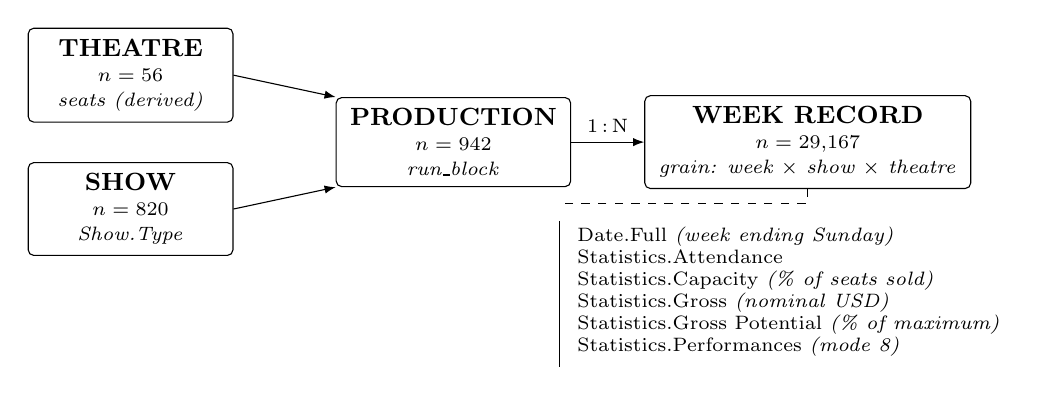
\begin{tikzpicture}[
  font=\small,
  box/.style={draw, rounded corners=2pt, minimum height=10mm, minimum width=26mm,
              inner xsep=5pt, inner ysep=4pt, align=center},
  attr/.style={font=\scriptsize, anchor=west},
  link/.style={draw, -{Latex[length=4pt]}, thin}
]
\node[box] (theatre) at (0,3.35)
  {\textbf{THEATRE}\\[-2pt]\scriptsize $n=56$\\[-2pt]\scriptsize \textit{seats (derived)}};
\node[box] (show) at (0,1.65)
  {\textbf{SHOW}\\[-2pt]\scriptsize $n=820$\\[-2pt]\scriptsize \textit{Show.Type}};
\node[box] (prod) at (4.1,2.50)
  {\textbf{PRODUCTION}\\[-2pt]\scriptsize $n=942$\\[-2pt]\scriptsize \textit{run\_block}};
\node[box] (week) at (8.6,2.50)
  {\textbf{WEEK RECORD}\\[-2pt]\scriptsize $n=29{,}167$\\[-2pt]\scriptsize \textit{grain: week $\times$ show $\times$ theatre}};

\draw[link] (theatre.east) -- (prod.north west);
\draw[link] (show.east)    -- (prod.south west);
\draw[link] (prod.east)    -- node[above, font=\scriptsize] {1\,:\,N} (week.west);

\node[attr, anchor=north west, align=left] (attrs) at (5.55,1.55)
  {Date.Full \textit{(week ending Sunday)} \\
   Statistics.Attendance \\
   Statistics.Capacity \textit{(\% of seats sold)} \\
   Statistics.Gross \textit{(nominal USD)} \\
   Statistics.Gross Potential \textit{(\% of maximum)} \\
   Statistics.Performances \textit{(mode 8)}};
\draw[thin] (5.45,1.50) -- (5.45,-0.35);
\draw[thin, dashed] (week.south) -- (8.6,1.72) -- (5.45,1.72);
\end{tikzpicture}
\caption{Entity structure recovered from the flat file. \code{PRODUCTION} is the
decision-making unit and the grouping unit for train/test splits; seat counts
are derived rather than supplied.}
\label{fig:datamodel}
\end{figure}

\begin{table}[htbp]
\centering
\caption{Data quality audit and cleaning decisions, implemented as
\code{CLEANING\_DECISIONS} in the data-loading module.}
\label{tab:quality}
\small
\begin{tabular}{@{}p{2.9cm}p{4.6cm}p{6.4cm}@{}}
\toprule
\textbf{Issue} & \textbf{Evidence} & \textbf{Decision} \\
\midrule
Coverage gaps &
29 weeks missing in 1990--91 and 42 in 1991--92; 75 missing weeks in total &
Restrict analysis to 1996 onward (28{,}479 rows); retain earlier years only as
a quality exhibit \\[3pt]

\code{Performances} $=0$ &
2{,}309 rows (7.9\%) report zero performances alongside positive attendance,
which is impossible &
Recode to \code{NaN}, flag \code{perf\_missing}; never impute \\[3pt]

\code{Gross Potential} $=0$ &
1{,}918 rows (6.6\%); 96\% of all 1996 rows are affected, and the defect
disappears entirely after 1997 &
Recode to \code{NaN}, flag \code{gp\_missing} \\[3pt]

\code{Capacity} censored &
Capped at 100\%, yet 1{,}433 rows show gross potential above 100\% from
premium pricing &
Treat 100 as right-censored; state the censoring wherever capacity is modelled \\[3pt]

Nominal currency &
Median ticket price rises 109\% between 1996 and 2015 &
Model scale-free measures (capacity \%, gross potential \%); carry \code{year}
as a feature; no external deflator \\[3pt]

Title-case artefacts &
42 of 820 titles contain \code{'S} from word-wise capitalisation &
Normalise to \code{'s}; retain the original in \code{show\_name\_raw} \\[3pt]

Multi-theatre titles &
27 titles run in more than one theatre &
Key productions on (show, theatre, run\_block) \\
\bottomrule
\end{tabular}
\end{table}

\begin{table}[htbp]
\centering
\caption{Horizon selection for Candidate 1. Persistence decays faster than the
model, so the model's contribution grows with the horizon. Test period 2015-01
to 2016-08; the majority-class baseline is 0.35 at every horizon. Bold marks the
better of baseline and model.}
\label{tab:horizon}
\small
\begin{tabular}{@{}lcccc@{}}
\toprule
& \multicolumn{2}{c}{\textbf{Accuracy (3 bands)}} & \multicolumn{2}{c}{\textbf{MAE (capacity \%)}} \\
\cmidrule(lr){2-3}\cmidrule(lr){4-5}
\textbf{Horizon} & Persistence & Logistic reg. & Persistence & Linear reg. \\
\midrule
1 week  & \textbf{0.728} & 0.724 & 5.52 & \textbf{5.33} \\
2 weeks & 0.634 & \textbf{0.656} & 7.21 & \textbf{6.52} \\
4 weeks & 0.607 & \textbf{0.638} & 8.01 & \textbf{7.36} \\
\bottomrule
\end{tabular}
\end{table}

\begin{table}[htbp]
\centering
\caption{Candidate problems against the brief's scoping checklist.}
\label{tab:checklist}
\small
\begin{tabular}{@{}p{2.7cm}p{4.0cm}p{3.7cm}p{3.4cm}@{}}
\toprule
\textbf{Criterion} & \textbf{C1 demand (4 weeks)} & \textbf{C2 closure risk} & \textbf{C3 opening gross} \\
\midrule
Derivable target & Yes, a column & Yes, from last observed week & Yes, weeks 1--4 \\
No leakage & Yes, lags start at $t{-}4$ & Yes, run state and lags & Yes, but no lags exist \\
Sufficient signal & 0.638 vs 0.315 / 0.607 & PR-AUC 0.698 vs 0.204 & $R^2 = 0.29$ (weak) \\
Manageable imbalance & Balanced by construction & 22\% positive; weights, PR-AUC & N/A (regression) \\
Clear stakeholder & Theatre GM & Producer & Marketing \\
\midrule
\textbf{Verdict} & \textbf{Primary} & \textbf{Secondary} & Deprioritised \\
\bottomrule
\end{tabular}
\end{table}

\begin{table}[htbp]
\centering
\caption{Data dictionary for \code{broadway\_clean.csv}. ``Coded missing''
records values that represent absent data rather than genuine measurements.}
\label{tab:dictionary}
\small
\begin{tabular}{@{}llp{6.1cm}l@{}}
\toprule
\textbf{Column} & \textbf{Type} & \textbf{Description} & \textbf{Coded missing} \\
\midrule
\code{Date.Full}   & date & Week-ending date; always a Sunday & --- \\
\code{Date.Day}    & int  & Day component of \code{Date.Full} & --- \\
\code{Date.Month}  & int  & Month component (1--12) & --- \\
\code{Date.Year}   & int  & Year component (1990--2016) & --- \\
\code{Show.Name}   & text & Show title, word-wise capitalised (820 distinct) & --- \\
\code{Show.Theatre}& text & Venue name (56 distinct) & --- \\
\code{Show.Type}   & cat  & Musical / Play / Special & --- \\
\code{Statistics.} & int  & Total tickets sold across all performances that & --- \\
\quad\code{Attendance} &  & week & \\
\code{Statistics.} & int  & \textbf{Percentage} of available seats sold, 10--100. & 100 = censored \\
\quad\code{Capacity} &    & Not a seat count; see Equation~\ref{eq:identity} & \\
\code{Statistics.} & int  & Weekly box-office revenue in \textbf{nominal} USD, & --- \\
\quad\code{Gross}  &      & not inflation-adjusted & \\
\code{Statistics.} & int  & Percentage of maximum achievable gross; exceeds & 1{,}918 zeros \\
\quad\code{Gross Potential} & & 100 under premium pricing (1{,}433 rows) & \\
\code{Statistics.} & int  & Performances given that week; mode 8, the standard & 2{,}309 zeros \\
\quad\code{Performances} &  & Broadway schedule & \\
\midrule
\multicolumn{4}{@{}l@{}}{\textit{Derived in \code{src/}, not present in the raw file:}} \\
\code{theatre\_seats} & int & Seat count recovered via Equation~\ref{eq:identity} & --- \\
\code{production\_id} & text & (show, theatre, run\_block) --- the decision unit & --- \\
\code{capacity\_lag}$k$ & float & Capacity $k$ weeks earlier, same production & gaps in run \\
\code{target\_band} & cat & Low / Mid / High, at training-set terciles & --- \\
\code{target\_closes\_soon} & bin & Closes within 8 weeks & 208 censored \\
\bottomrule
\end{tabular}
\end{table}

\newpage
\section{Figures}
\label{app:figures}

\begin{figure}[htbp]
  \centering
  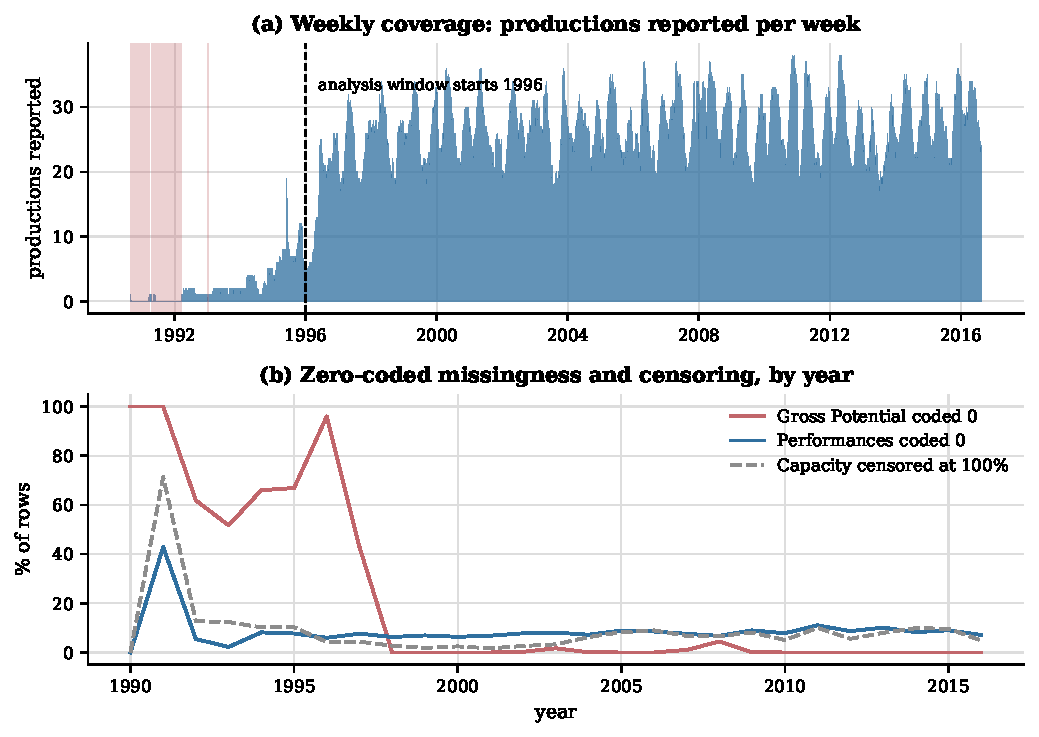
\includegraphics[width=\linewidth]{fig01_data_quality.pdf}
  \caption{Data quality. (a) Productions reported per week; shaded bands are the
  four coverage gaps, totalling 75 missing weeks. (b) Share of rows affected by
  zero-coded missingness and by censoring, per year. Both defects are era
  effects rather than show effects, which is why the analysis window starts in
  1996.}
  \label{fig:quality}
\end{figure}

\begin{figure}[htbp]
  \centering
  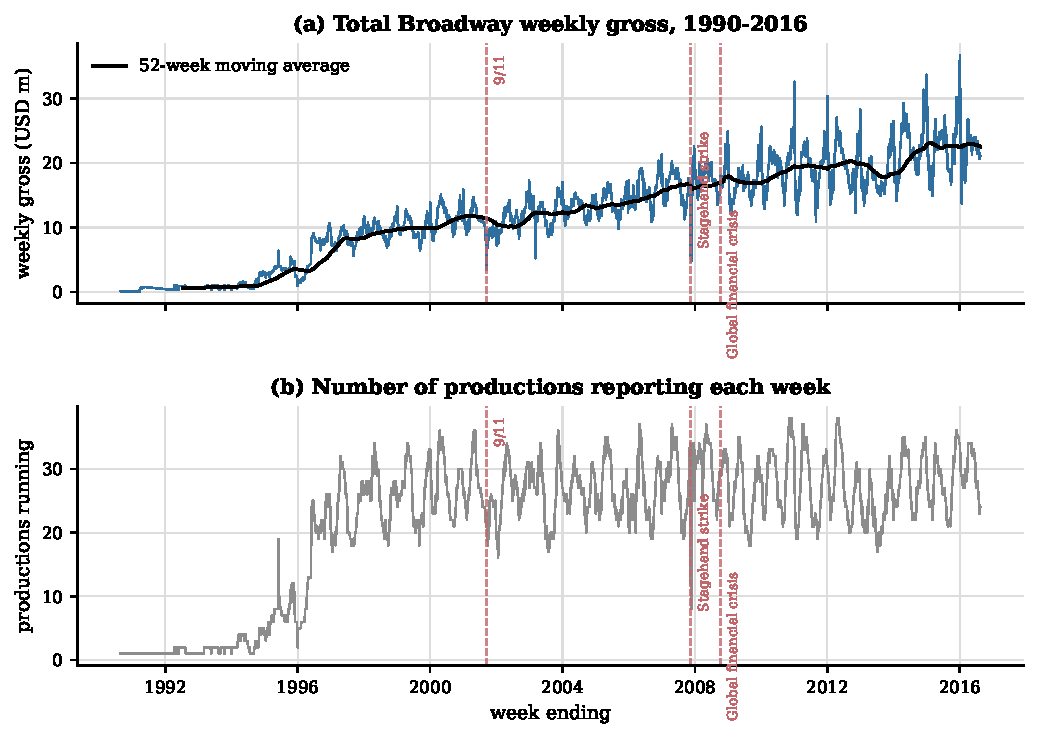
\includegraphics[width=\linewidth]{fig02_market_events.pdf}
  \caption{Total Broadway weekly gross and the number of productions reporting,
  1990--2016, with the three exogenous shocks marked. The stagehands' strike is
  visible in both panels; the 9/11 collapse is a revenue effect without a
  corresponding fall in the number of productions.}
  \label{fig:market}
\end{figure}

\begin{figure}[htbp]
  \centering
  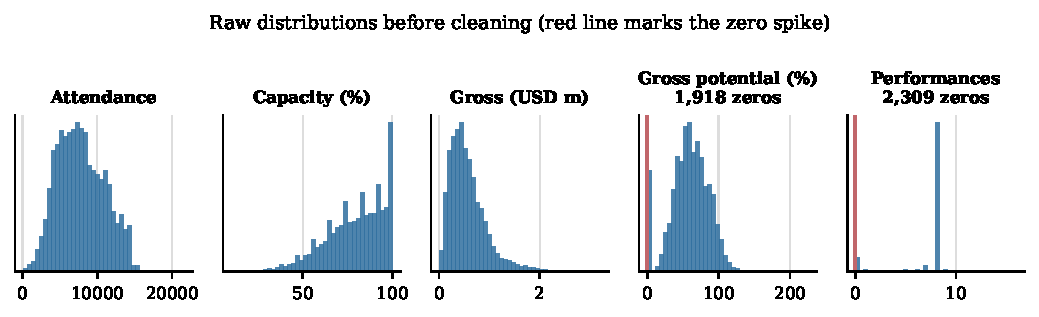
\includegraphics[width=\linewidth]{fig04_distributions.pdf}
  \caption{Raw distributions before cleaning. The red line marks the spike at
  zero in \code{Performances} and \code{Gross Potential}: these are missing
  values encoded as zero, not genuine observations.}
  \label{fig:distributions}
\end{figure}

\begin{figure}[htbp]
  \centering
  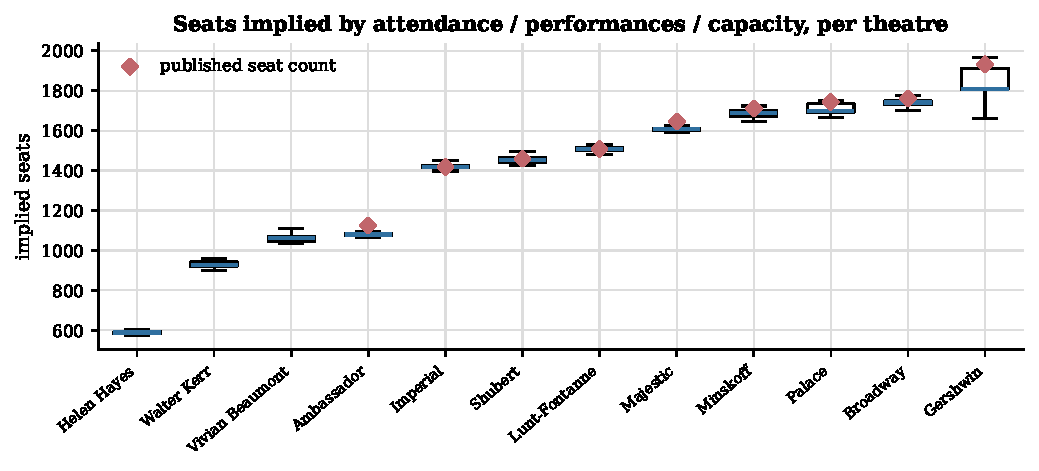
\includegraphics[width=\linewidth]{fig05_capacity_validation.pdf}
  \caption{Validating the meaning of \code{Statistics.Capacity}. Boxplots show
  the seat count implied by
  $\text{attendance}/\text{performances}\,/\,(\text{capacity}/100)$ for each
  theatre; diamonds are published seat counts. The implied values are tight
  within a theatre and match the published figures to a median error of
  1.7\%, establishing that the column is a percentage.}
  \label{fig:validation}
\end{figure}

\begin{figure}[htbp]
  \centering
  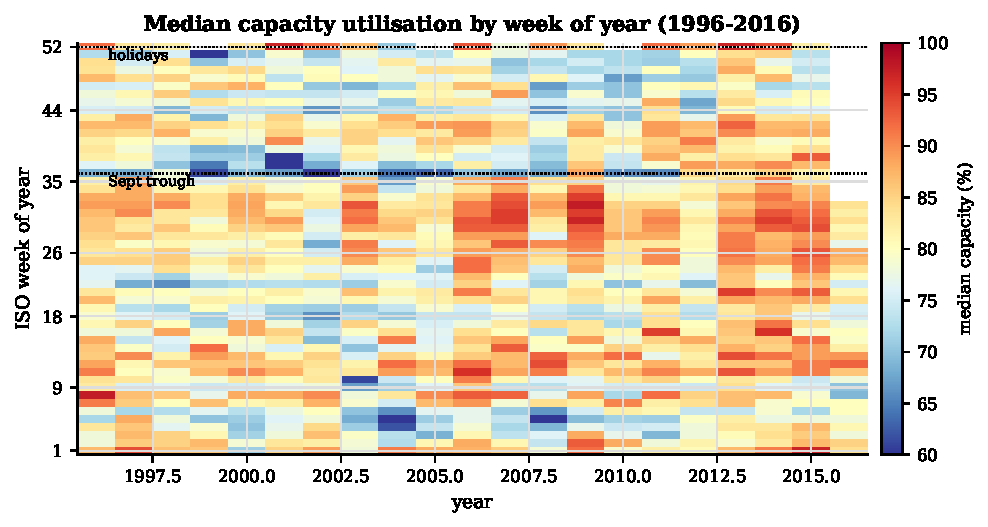
\includegraphics[width=\linewidth]{fig06_seasonality.pdf}
  \caption{Median capacity utilisation by ISO week and year. The holiday band at
  weeks 52--53 and the September trough near week 36 persist across all
  twenty-one seasons.}
  \label{fig:seasonality}
\end{figure}

\begin{figure}[htbp]
  \centering
  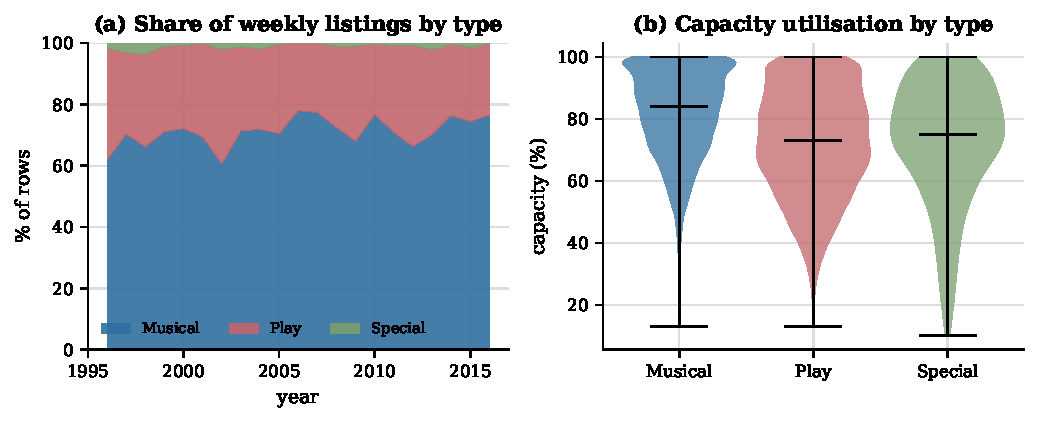
\includegraphics[width=\linewidth]{fig07_show_types.pdf}
  \caption{(a) Composition of weekly listings by show type. (b) Distribution of
  capacity utilisation by type. Musicals dominate the panel and sustain higher
  utilisation than plays.}
  \label{fig:types}
\end{figure}

\begin{figure}[htbp]
  \centering
  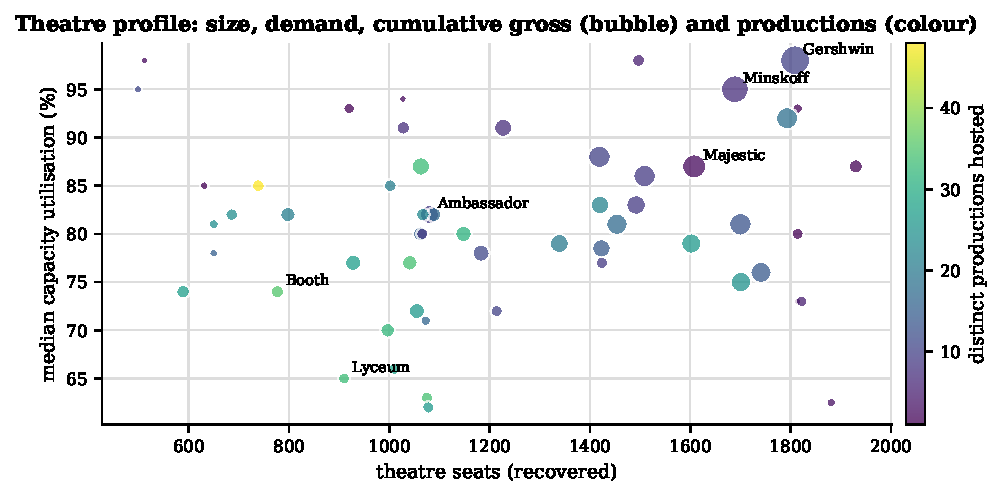
\includegraphics[width=\linewidth]{fig08_theatres.pdf}
  \caption{Theatre profile: recovered seat count against median capacity
  utilisation, sized by cumulative gross and coloured by the number of distinct
  productions hosted. Larger houses are not systematically fuller houses.}
  \label{fig:theatres}
\end{figure}

\begin{figure}[htbp]
  \centering
  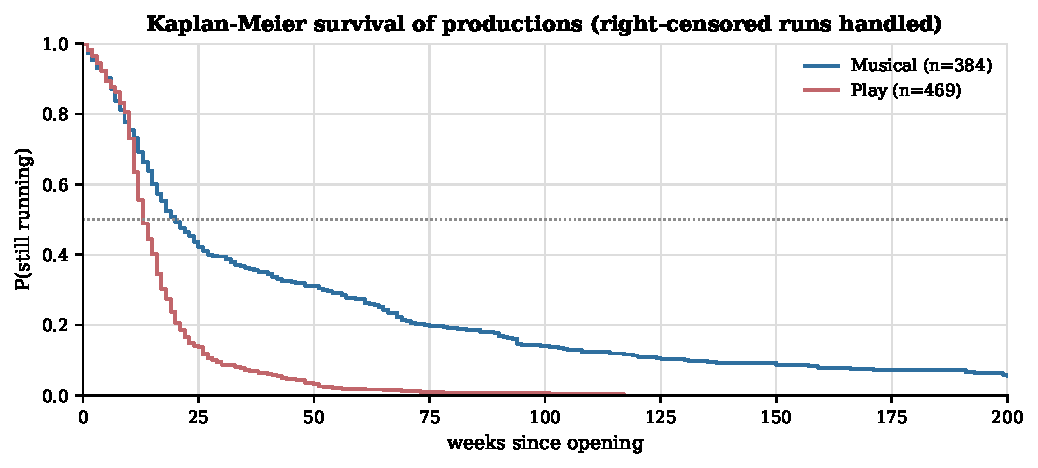
\includegraphics[width=\linewidth]{fig09_survival.pdf}
  \caption{Kaplan--Meier survival curves for productions by show type, with
  right-censored runs handled explicitly. Median survival is 20 weeks for
  musicals and 13 weeks for plays.}
  \label{fig:survival}
\end{figure}

\begin{figure}[htbp]
  \centering
  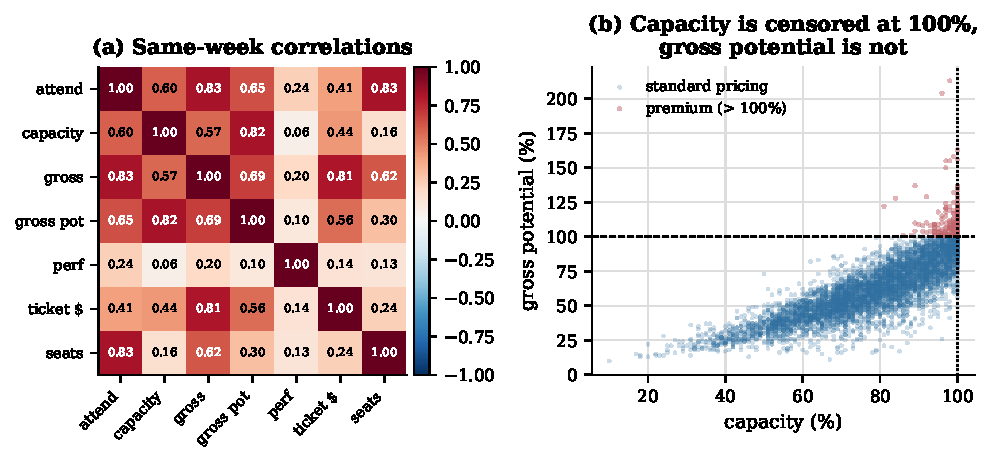
\includegraphics[width=\linewidth]{fig10_relationships.pdf}
  \caption{(a) Same-week correlations. (b) Capacity against gross potential.
  Capacity is censored at 100\% whereas gross potential is not, so premium
  pricing pushes 1{,}433 observations above the 100\% line.}
  \label{fig:relationships}
\end{figure}

\begin{figure}[htbp]
  \centering
  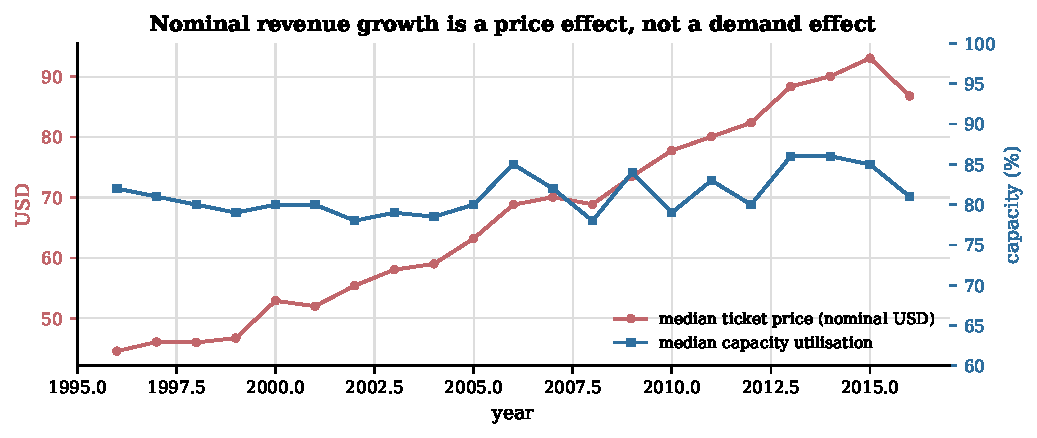
\includegraphics[width=\linewidth]{fig11_price_vs_demand.pdf}
  \caption{Median nominal ticket price against median capacity utilisation.
  Price rises 109\% between 1996 and 2015 while utilisation moves three
  percentage points: growth in nominal gross is overwhelmingly a price effect.}
  \label{fig:price}
\end{figure}

\begin{figure}[htbp]
  \centering
  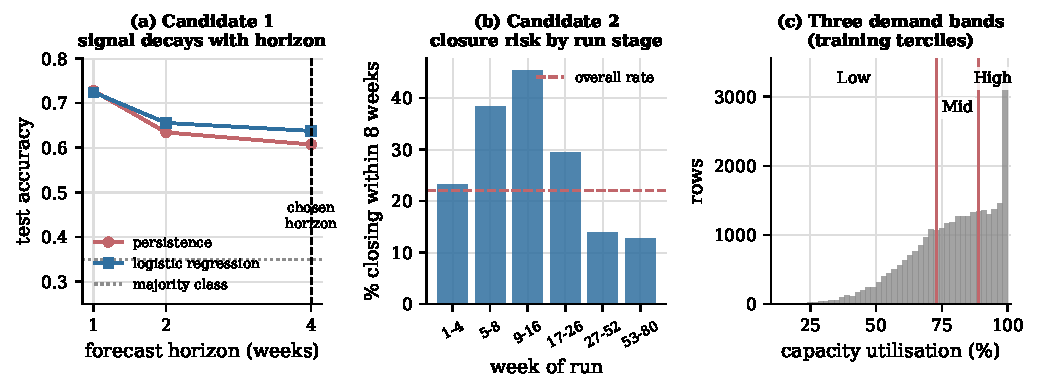
\includegraphics[width=\linewidth]{fig12_candidates.pdf}
  \caption{Candidate problem evidence. (a) Accuracy against forecast horizon:
  persistence decays faster than the model, so the model's contribution grows
  with the horizon. (b) Closure risk by stage of run. (c) The demand bands,
  defined by training-set terciles.}
  \label{fig:candidates}
\end{figure}

\end{document}
